% Activate the following line by filling in the right side. If for example the name of the root file is Main.tex, write
% "...root = Main.tex" if the chapter file is in the same directory, and "...root = ../Main.tex" if the chapter is in a subdirectory.
 
%!TEX root =  dissertation.tex

\chapter[Analysis]{Analysis}

\section{Usability result and analysis}

Usability evaluation is done using online survey hosted by Google Form\footnote{\url{https://goo.gl/forms/toYsRwnGIGumMBUD2}}. Respondents are given 2 tasks to complete, which are to run a simulation and reproduce past simulation. I analyze respondent's answers with regards to HemeWeb's usability.


\subsection{Demography}


\vspace{1cm}

\noindent%
\begin{minipage}{\linewidth}% to keep image and caption on one page
\makebox[\linewidth]{
  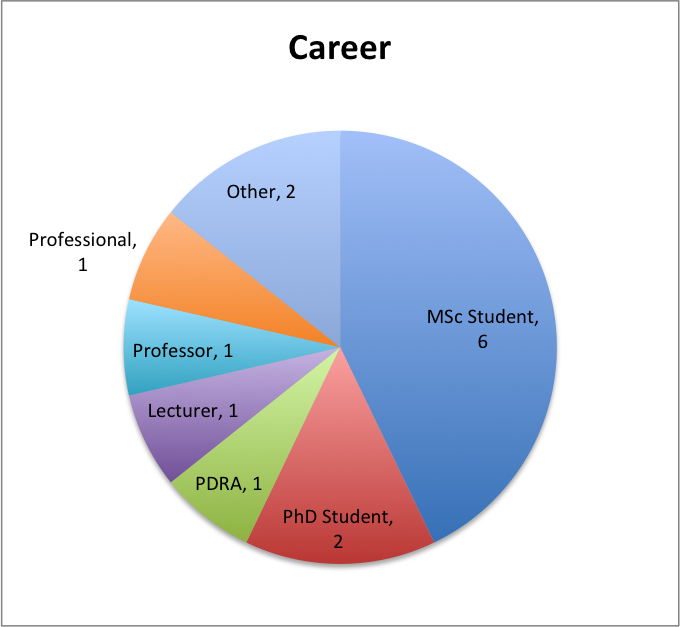
\includegraphics[keepaspectratio=true,scale=0.8]{../resources/evaluation/usability/career.png}
 }
\captionof{figure}{Career stage distribution} \label{fig:survey-career}%      only if needed  
\end{minipage}

\vspace{1cm}

\vspace{1cm}

\noindent%
\begin{minipage}{\linewidth}% to keep image and caption on one page
\makebox[\linewidth]{
  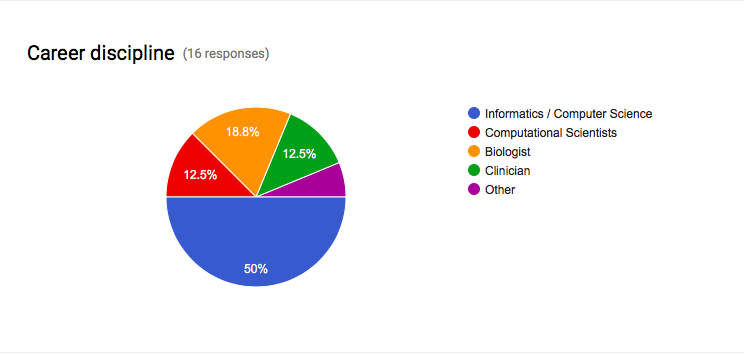
\includegraphics[keepaspectratio=true,scale=0.8]{../resources/evaluation/usability/discipline.png}
 }
\captionof{figure}{Career discipline} \label{fig:survey-discipline}%      only if needed  
\end{minipage}

\vspace{1cm}


The survey was filled by 16 respondents over the period of 10 days (3rd August 2016 - 10th August 2016). However, because 1 of the respondent are unable to run the tasks, we remove the reponse because it will not add any meaningful information. In the end we have 15 valid respondents. We can classify the respondents with their career stage and discipline. From here, we can classify the respondents from informatics / computer science related discipline or not. From figure \ref{fig:survey-career} and \ref{fig:survey-discipline}, around 62.5\% of the respondents are either informatics or computational scientists, while 37.3\% can be considered domain experts (Biologist, Clinician, and Biophysicist)

\vspace{1cm}

\noindent%
\begin{minipage}{\linewidth}% to keep image and caption on one page
\makebox[\linewidth]{
  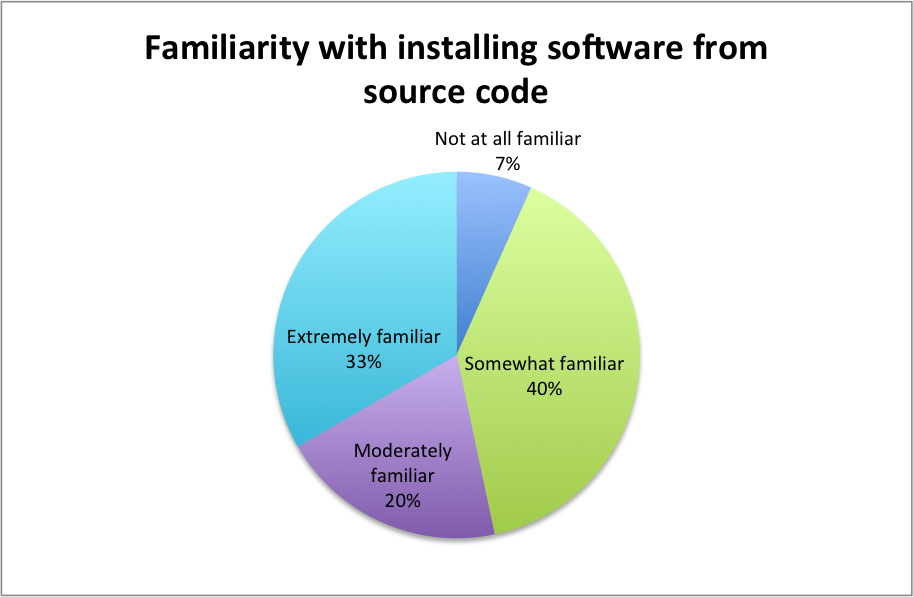
\includegraphics[keepaspectratio=true,scale=0.8]{../resources/evaluation/usability/source_code.png}
 }
\captionof{figure}{Familiarity with installing software from source code} \label{fig:survey-source}%      only if needed  
\end{minipage}

\vspace{1cm}

\noindent%
\begin{minipage}{\linewidth}% to keep image and caption on one page
\makebox[\linewidth]{
  
\includegraphics[keepaspectratio=true,scale=0.8]{../resources/evaluation/usability/browser.png}
 }
\captionof{figure}{Familiarity with web browser} \label{fig:survey-browser}%      only if needed  
\end{minipage}

\vspace{1cm}

\noindent%
\begin{minipage}{\linewidth}% to keep image and caption on one page
\makebox[\linewidth]{
  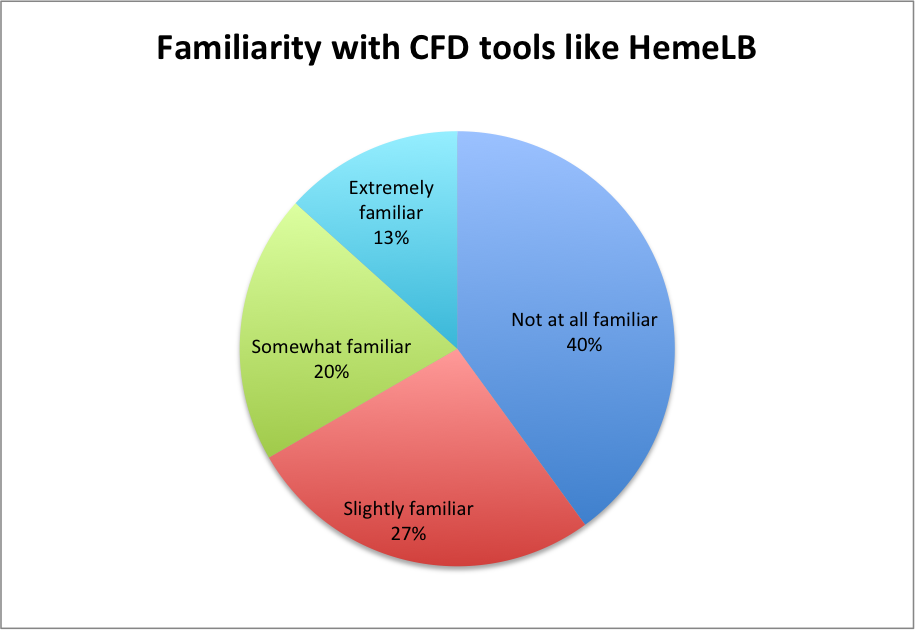
\includegraphics[keepaspectratio=true,scale=0.8]{../resources/evaluation/usability/hemelb.png}
 }
\captionof{figure}{Familiarity with CFD tools like HemeLB} \label{fig:survey-hemelb}%      only if needed  
\end{minipage}

\vspace{1cm}


We can also further classify the respondents based on the familiarity with browsers, computational fluid dynamic tools, and installing software from source code. All of this are shown in Figure \ref{fig:survey-source}, \ref{fig:survey-browser}, and \ref{fig:survey-hemelb}.




\subsection{Scenario 1: Run a simulation}

To measure the usability of HemeWeb for users to run a simulation, respondents were asked to run a  scenario. Instructions to run a HemeLB simulation were provided and they were asked to follow it to produce a simulation. Respondents then were asked to state their agreement with three statements which are provided. These three questions measure how usable HemeWeb is to them. 


\vspace{1cm}

\noindent%
\begin{minipage}{\linewidth}% to keep image and caption on one page
\makebox[\linewidth]{
  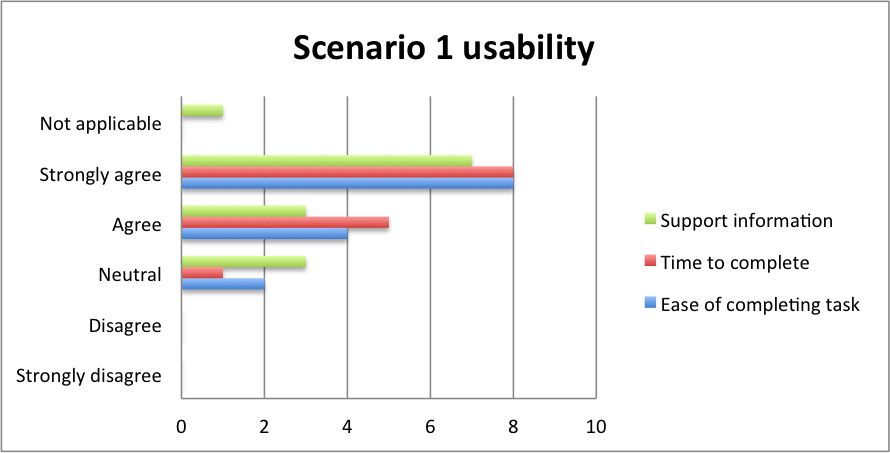
\includegraphics[keepaspectratio=true,scale=0.9]{../resources/evaluation/usability/scenario1_usability.png}
 }
\captionof{figure}{Scenario 1 usability} \label{fig:survey-s1-usability}%      only if needed  
\end{minipage}

On Figure \ref{fig:survey-s1-usability}, the responses is shown. Generally, respondents tend to agree that HemeWeb are usable to run a simulation from the three statements. However, one respondent fill out Not applicable towards the statement that says they are satisfied with support information HemeWeb give them. This could means that the respondent doesn't feel the scenario give enough information for them to agree or disagree with the statements.

Based on the responses, we can also deduce the system's usability in running a simulation by calculating the After Scenario Questionnare score, or ASQ score. We assign an integer value, 1 for Strongly disagree, 2 for disagree, 3 for neutral, 4 for Agree, and 5 for strongly disagree. Next, we take the mean of the values for each questions and ignore the answer with Not Applicable to determine a single ASQ score for that respondent. With this schema we can determine that for the respondents tend to agree that they are satisfied with the usability of the system with the overall ASQ score of 4.36

Our hypothesis is that users will generally find using web interface is usable and the data seemed to support that. It is much easier for user to complete a task when using point and click interface rather than requiring them to recall commands to do the tasks, especially when they are not familiar with the tools.


Next, respondents are given a high overview of replicating the tasks done in HemeWeb but using command line interface. Respondents are not asked to run the scenario in their command line interface because we cannot make sure the necessary tools are installed on respondent's computer.

\vspace{1cm}

\noindent%
\begin{minipage}{\linewidth}% to keep image and caption on one page
\makebox[\linewidth]{
  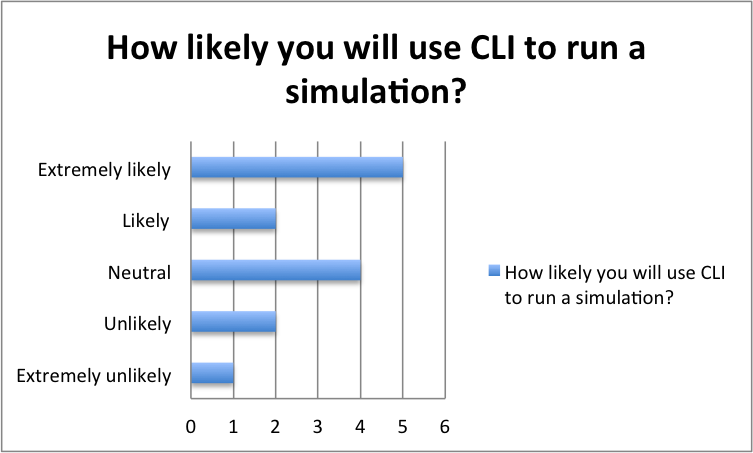
\includegraphics[keepaspectratio=true,scale=0.9]{../resources/evaluation/usability/scenario1_cli.png}
 }
\captionof{figure}{Scenario 1 command line preference} \label{fig:survey-s1-cli}%      only if needed  
\end{minipage}

\vspace{1cm}

\noindent%
\begin{minipage}{\linewidth}% to keep image and caption on one page
\makebox[\linewidth]{
  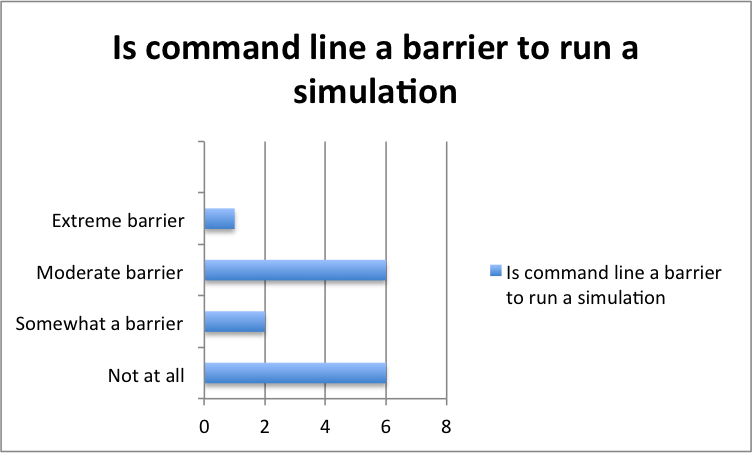
\includegraphics[keepaspectratio=true,scale=0.9]{../resources/evaluation/usability/scenario1_cli_barrier.png}
 }
\captionof{figure}{Scenario 1 barrier in using command line} \label{fig:survey-s1-cli-barrier}%      only if needed  
\end{minipage}

\vspace{1cm}

Figure \ref{fig:survey-s1-cli} and \ref{fig:survey-s1-cli-barrier} shows the general sentiment of users in running the simulation but in the command line. From the data, respondents are generally open to the likelihood of them running the simulation using command line, if we quantify the response, it got the score of 3.46, somewhere between neutral and likely. However, when we realize that the the 62.5\% of the respondent has background in informatics / computational scientists who deal a lot with command line, this become clearer.

Our hypothesis is that domain experts would most likely find CLI a barrier to run a simulation and ess likely to run simulation with it.



\subsection{Scenario 2: Reproduce past simulation}

\vspace{1cm}

\noindent%
\begin{minipage}{\linewidth}% to keep image and caption on one page
\makebox[\linewidth]{
  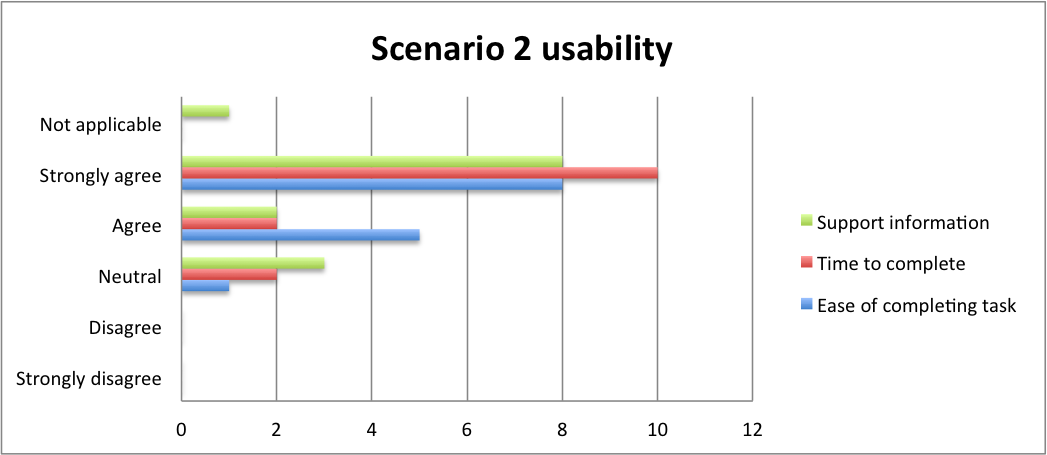
\includegraphics[keepaspectratio=true,scale=0.9]{../resources/evaluation/usability/scenario2_usability.png}
 }
\captionof{figure}{Scenario 2 usability} \label{fig:survey-s2-usability}%      only if needed  
\end{minipage}

\vspace{1cm}

\noindent%
\begin{minipage}{\linewidth}% to keep image and caption on one page
\makebox[\linewidth]{
  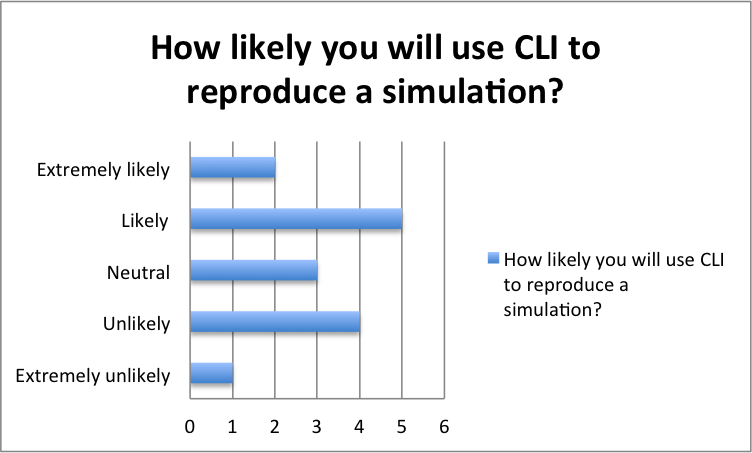
\includegraphics[keepaspectratio=true,scale=0.9]{../resources/evaluation/usability/scenario2_cli.png}
 }
\captionof{figure}{Scenario 2 command line preference} \label{fig:survey-s2-cli}%      only if needed  
\end{minipage}

\vspace{1cm}

\noindent%
\begin{minipage}{\linewidth}% to keep image and caption on one page
\makebox[\linewidth]{
  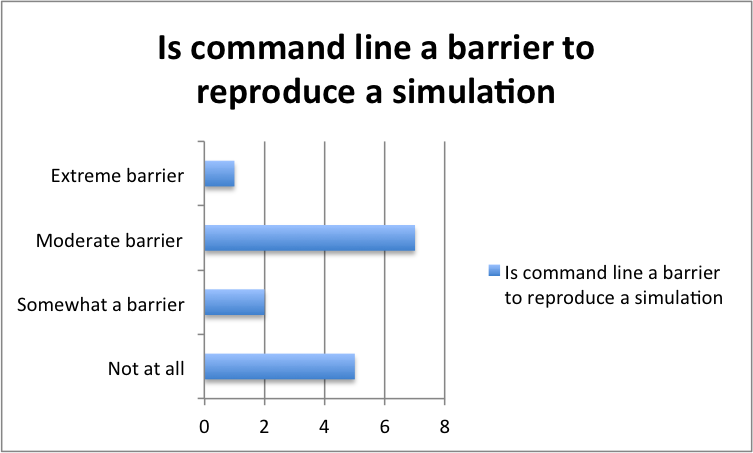
\includegraphics[keepaspectratio=true,scale=0.9]{../resources/evaluation/usability/scenario2_cli_barrier.png}
 }
\captionof{figure}{Scenario 2 barrier in using command line} \label{fig:survey-s2-cli-barrier}%      only if needed  
\end{minipage}

\vspace{1cm}



\subsection{Overall usability}


Here, I will discuss the overall usability of the system using the post study system usability questionnaire as the basis. This questionnaire consists of 19 questions and can be divided into measuring three different part. They are system usefulness, information quality, and the interface quality. I will discuss each of them in details.

%%%%%%%%%%%%%%%%%%%%%%%%%%%%%%%%%%%
%  SYSTEM USEFULNESS 
%%%%%%%%%%%%%%%%%%%%%%%%%%%%%%%%%%%
\begin{center}
\captionof{table}{System usefulness}\label{table:overall-usability}
\scalebox{0.75}{

\begin{tabular}{|l|l|l|l|l|l|l|}
\hline
                                                                                                          & \begin{tabular}[c]{@{}l@{}}Strongly \\ disagree\end{tabular} & Disagree & Neutral & Agree & \begin{tabular}[c]{@{}l@{}}Strongly \\ agree\end{tabular} & \begin{tabular}[c]{@{}l@{}}Not \\ applicable\end{tabular} \\ \hline
\begin{tabular}[c]{@{}l@{}}Overall, I am satisfied with\\  how easy it is to use this system\end{tabular} & 0                                                            & 0        & 0       & 8     & 7                                                         & 0                                                         \\ \hline
It was simple to use this system                                                                          & 0                                                            & 0        & 0       & 2     & 13                                                        & 0                                                         \\ \hline
I can effectively complete my work using this system                                                      & 1                                                            & 1        & 2       & 3     & 4                                                         & 4                                                         \\ \hline
I am able to complete my work quickly using this system                                                   & 0                                                            & 1        & 3       & 3     & 6                                                         & 2                                                         \\ \hline
I am able to efficiently complete my work using this system                                               & 0                                                            & 2        & 2       & 4     & 5                                                         & 2                                                         \\ \hline
I feel comfortable using this system                                                                      & 1                                                            & 1        & 0       & 3     & 10                                                        & 0                                                         \\ \hline
It was easy to learn to use this system                                                                   & 0                                                            & 0        & 2       & 0     & 13                                                        & 0                                                         \\ \hline
I believe I became productive quickly using this system                                                   & 0                                                            & 1        & 2       & 3     & 5                                                         & 4                                                         \\ \hline
\end{tabular}
}
\end{center}
\vspace{1cm}

Table \ref{table:overall-usability} shows the respondents sentiment towards the system usefulness. Generally, we can see the distribution that people tend to agree to the 9 statements presented to them. If we convert the response into a numerical value, we can get the score of 4.27 of system usefulness, which is quite high. However, there are still some improvements that can be made, and it is apparent in the feedbacks of the system we got. In addition, there are respondents that respond to the statement by answering Not applicable. It is mostly on the framing of the simulation as a 'work'. Respondents might have no point of reference whether using the HemeLb via HemeWeb is quicker or efficiently because they are new to the system. It is apparent that from their background they don't  have familiarity with HemeLB.


%%%%%%%%%%%%%%%%%%%%%%%%%%%%%%%%%%%
%  INFO QUALITY
%%%%%%%%%%%%%%%%%%%%%%%%%%%%%%%%%%%

\begin{center}
\captionof{table}{Information quality}\label{table:overall-info-quality}
\scalebox{0.75}{
\begin{tabular}{|l|l|l|l|l|l|l|}
\hline
                                                                                                                                                                               & \begin{tabular}[c]{@{}l@{}}Strongly\\ disagree\end{tabular} & Disagree & Neutral & Agree & \begin{tabular}[c]{@{}l@{}}Strongly\\ agree\end{tabular} & \begin{tabular}[c]{@{}l@{}}Not\\ applicable\end{tabular} \\ \hline
\begin{tabular}[c]{@{}l@{}}The system gives error messages that\\  clearly tell me how to fix problems\end{tabular}                                                            & 0                                                           & 2        & 1       & 4     & 2                                                        & 6                                                        \\ \hline
\begin{tabular}[c]{@{}l@{}}Whenever I make a mistake using the system, \\ I recover easily and quickly\end{tabular}                                                            & 0                                                           & 0        & 5       & 1     & 3                                                        & 6                                                        \\ \hline
\begin{tabular}[c]{@{}l@{}}The information (such as online help, \\ on-screen messages, and other documentation)\\  provided with this system is clear\end{tabular}            & 0                                                           & 0        & 3       & 4     & 5                                                        & 3                                                        \\ \hline
It is easy to find the information I needed                                                                                                                                    & 0                                                           & 1        & 2       & 3     & 6                                                        & 3                                                        \\ \hline
\begin{tabular}[c]{@{}l@{}}The information (such as online help,\\  on-screen messages, and other documentation)\\  provided for the system is easy to understand\end{tabular} & 0                                                           & 1        & 2       & 5     & 6                                                        & 1                                                        \\ \hline
\begin{tabular}[c]{@{}l@{}}The information is effective in helping me\\  complete the tasks and scenarios\end{tabular}                                                         & 0                                                           & 1        & 4       & 2     & 7                                                        & 1                                                        \\ \hline
\begin{tabular}[c]{@{}l@{}}The organization of information on the \\ system screens is clear\end{tabular}                                                                      & 0                                                           & 0        & 3       & 8     & 4                                                        & 0                                                        \\ \hline
\end{tabular}

}
\end{center}
\vspace{1cm}

On the information quality side of things, we also find similar results with regards to the sentiment of the respondents. From the 7 statements that we presented, most respondents to agree that the information quality tends to be good. However, There are a lot of respondents filling in Not applicable. However the overall sentiment is good. When we convert it to the number, we got 4.0 average score that tells that overall respondents find the information quality quite good. The organization of information,  the ease to find such information tends to be generally good.



%%%%%%%%%%%%%%%%%%%%%%%%%%%%%%%%%%%
%  INTERFACE QUALITY
%%%%%%%%%%%%%%%%%%%%%%%%%%%%%%%%%%%
\begin{center}
\captionof{table}{Interface quality}\label{table:overall-interface-quality}
\scalebox{0.75}{
\begin{tabular}{|l|l|l|l|l|l|l|}
\hline
                                                                                                                  & \begin{tabular}[c]{@{}l@{}}Strongly\\ disagree\end{tabular} & Disagree & Neutral & Agree & \begin{tabular}[c]{@{}l@{}}Strongly\\ agree\end{tabular} & \begin{tabular}[c]{@{}l@{}}Not\\ applicable\end{tabular} \\ \hline
The interface of this system is pleasant                                                                          & 1                                                           & 1        & 1       & 7     & 5                                                        & 0                                                        \\ \hline
I like using the interface of this system                                                                         & 0                                                           & 2        & 1       & 8     & 4                                                        & 0                                                        \\ \hline
\begin{tabular}[c]{@{}l@{}}This system has all the functions and\\  capabilities I expect it to have\end{tabular} & 1                                                           & 2        & 1       & 4     & 4                                                        & 3                                                        \\ \hline
\end{tabular}
}
\end{center}
\vspace{1cm}


On the interface quality, we started to see respondents answering with strongly disagree with positive statements about the interface. While in general, respondents find the interface of the system is good, some find it not. When we see the answer of this particular response, it seemed that the respondent had trouble with the interface not rendering correctly in firefox. This means that the user interface might not achieve web browser compatibility yet. However, in general, we find more people gravitates toward agreeing about the interface being good. All of this can be seen in Table \ref{table:overall-interface-quality}


\begin{center}
\captionof{table}{Overall user satisfaction quality}\label{table:overall-satisfaction}
\scalebox{0.75}{
\begin{tabular}{|l|l|l|l|l|l|l|}
\hline
                                         & \begin{tabular}[c]{@{}l@{}}Strongly\\ disagree\end{tabular} & Disagree               & Neutral                & Agree                  & \begin{tabular}[c]{@{}l@{}}Strongly\\ agree\end{tabular} & \begin{tabular}[c]{@{}l@{}}Not\\ applicable\end{tabular} \\ \hline
Overall, I am satisfied with this system & \multicolumn{1}{c|}{0}                                      & \multicolumn{1}{c|}{0} & \multicolumn{1}{c|}{2} & \multicolumn{1}{c|}{7} & \multicolumn{1}{c|}{6}                                   & \multicolumn{1}{c|}{0}                                   \\ \hline
\end{tabular}
}
\end{center}
\vspace{1cm}

The last part of the question is the overall perceived satisfaction that the user has in using the system. The distribution of the response can be found in Table \ref{table:overall-satisfaction}. Most of the respondents gravitate towards agreeing and strongly agreeing that they are satisfied with the system. When we convert it into a numerical mean, it is 4.26, which is between agree and strongly agree. To get the overall user satisfaction score of the study, we average the numerical score between the 19 questions and we got 4.1. This means that the respondents mostly agree that they are satisfied with how the system performs, inform, and looks like.

\section{Performance result and analysis}

In this section, I will discuss the performance benchmark of HemeLB simulation done in ARCHER supercomputer, INDY2 HPC cluster, and AWS EC2 where HemeWeb is deployed to. HemeLB produced a report files that can be used to benchmark the performance of the simulation execution. I made sure that on each infrastructure, the input file we used is the same. I took the simulation total time result from that files and compare the value between infrastructure.


\begin{center}

\captionof{table}{Performance comparison HemeLB on INDY2 vs AWS EC2}\label{table:perf}

\begin{tabular}{|c|c|c|}
\hline
\multicolumn{1}{|l|}{}            & \multicolumn{2}{c|}{Performance in seconds}               \\ \hline
\multicolumn{1}{|c|}{\# of Cores} & \multicolumn{1}{c|}{INDY2} & \multicolumn{1}{c|}{AWS EC2} \\ \hline
36                                & 24.7                       & 36.3                         \\ \hline
72                                & 12.7                       & 29.9                         \\ \hline
144                               & 7.08                       & 36.5                         \\ \hline
288                               & 3.44                       & 32.4                         \\ \hline
576                               & 1.81                       & 20.4                         \\ \hline
1152                              & 1.58                       & N/A                             \\ \hline
\end{tabular}

\end{center}



\vspace{1cm}

\begin{center}
\captionof{table}{HemeLB performance on ARCHER supercomputer}\label{table:perf-archer}
\begin{tabular}{|c|c|c|}
\hline
\multicolumn{1}{|l|}{}            & \multicolumn{1}{c|}{Performance in seconds}               \\ \hline
\multicolumn{1}{|l|}{\# of Cores} & \multicolumn{1}{c|}{ARCHER}  \\ \hline
24                                & 29.2                                           \\ \hline
48                                & 21.5                                         \\ \hline
96                               & 15.7                                       \\ \hline
192                               & 37.3                                           \\ \hline
384                               & 38.5                                               \\ \hline
768                              & 12                                              \\ \hline
1536                              & 16.1                                              \\ \hline
\end{tabular}
\end{center}


\vspace{1cm}

\noindent%
\begin{minipage}{\linewidth}% to keep image and caption on one page
\makebox[\linewidth]{
  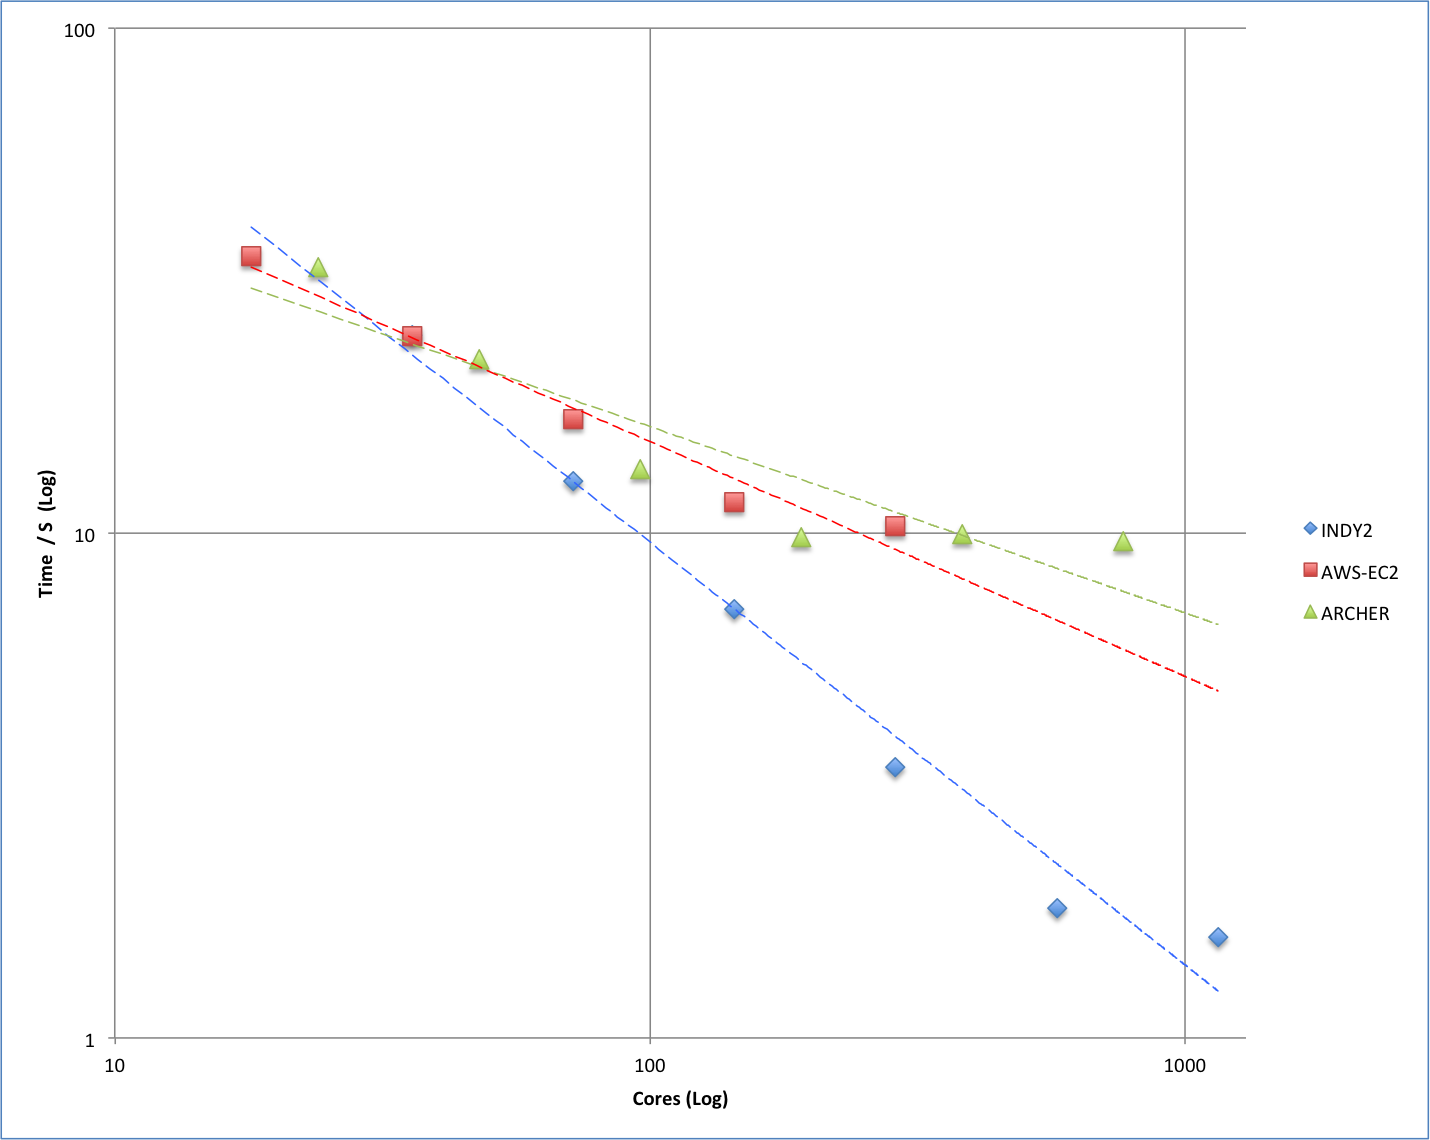
\includegraphics[keepaspectratio=true,scale=0.75]{../resources/evaluation/performance/overview.png}
 }
\captionof{figure}{HemeLB performance comparison} \label{fig:hemelb-perf-overview}%      only if needed  
\end{minipage}

\vspace{1cm}


In general, the performance of HemeLB with cloud infrastructure is worse when compared to ARCHER and INDY2. On each simulation instances with a different number of cores, we see slower simulation execution result when compared to the likes of the INDY2 machine and ARCHER supercomputer as observed on table \ref{table:perf}, \ref{table:perf-archer} and figure \ref{fig:hemelb-perf-overview}.

For the simulation, we use an input file which has 4,520,681 fluid sites. According to the performance analysis by Groen et al. \citep{groen2013analysing}, HemeLB scales up near-linearly up to 32,768 cores. It also performs near its maximum efficiency when using 5,000 to 500,000 sites per core. This means that for the problem size we use, HemeLB should perform near maximum efficiency when using 9 cores up to 900 cores. Above that core counts, HemeLB simulation will incur a performance penalty.

The simulation time of INDY2 as observed in Figure \ref{fig:hemelb-perf-overview} follows this performance model accurately. It scales almost linearly up to 576 cores, and finally hit a performance degradation on 1152 cores. However, the result on AWS-EC2 shows that HemeLB hits performance degradation much early that it does not follow the performance models. The reason being is that the infrastructure has an underlying difference in the networking capabilities. AWS-EC2 offer 10 Gigabit per second interface \footnote{\url{https://aws.amazon.com/premiumsupport/knowledge-center/network-throughput-benchmark-linux-ec2/}} while dedicated HPC infrastructure often uses InfiniBand or Cray Aries router interconnectivity which provides higher throughput \cite{Quan:2014aa}. This result is in line with the benchmark that Mehrotra et al. did on NASA's HPC application \citep{mehrotra2012performance}. The performance degradation comes from the network and the virtualization overhead that this cloud platform has. 


ARCHER supercomputer has slower simulation time compared to INDY2, because of the difference of processors used in the compute node. ARCHER used a three-year-old 2.7 GHz, 12-core E5-2697 v2 Ivy Bridge processor. Compared to INDY2 which boasts the newer Broadwell-based Intel Xeon CPU E5-2695 v4 @ 2.10GHz. The number of thread inside those processors also differ, ARCHER has 24 while INDY2 has 36. This makes the performance difference. On the other hand for this evaluation, we use Amazon's c4.8xlarge EC2 instance which has Haswell-based E5-2666 v3 processor that has 36 virtual CPU cores. All these difference contributes toward the speed difference oh the simulation results.

The scaling of the performance is where HemeWeb took a dive. It is apparent that with increased compute node, the network activity between the nodes become a bottleneck in the HemeWeb's case. The performance dip when we started the simulation using 4 compute nodes which have 144 cores that it is slower than just using 1 compute node. However, the performance improves as we add more compute nodes. This is not seen in the case of INDY2, where it scales very well and reach a diminishing return on the performance after using more than 1,000 cores.

\subsection{Price performance analysis}

To analyze the performance even further, we can compare the performance we get with the price we have to pay to run the infrastructure. In running the simulation for benchmark, we used c4.8xlarge linux instances on EU Ireland region which at the time of writing costs GBP 1.51\footnote{USD 1.96 converted to GBP on https://\url{www.oanda.com/currency/converter/} at 13th August 2016} per hour\footnote{\url{https://aws.amazon.com/ec2/pricing/}}. Phase 2 XC30 ARCHER supercomputer give access to screened project by compute hour which has the price of GBP 0.56 for research council which are partnered and GBP 1.33 for  non-partnered research council\footnote{Calculated on \url{http://archer.ac.uk/access/au-calculator/}}. INDY2 however have no public pricing released by the EPCC yet.

With these pricing information, we can deduce that using AWS EC2 is 2.69 times more expensive compared to using ARCHER with partnership and 1.13 times more expensive without partnership. With more costs, using HemeWeb has lower performance but comparable to the ARCHER supercomputer.  However, because there are no price information yet on INDY2, we cannot make any price performance comparison between AWS-EC2 with INDY2 that has bigger performance gap.

All of this performance pricing analysis however have to take into account of the model of business of the governing institution. On using Amazon's resources, one does not have to submit a proposal or go to a resource allocation community, he / she just need a credit cards and access will be given. In addition to that, Amazon employ the pay-as-you-go pricing scheme so it is very flexible in changing requirements or usage compared to ARCHER which allocate the resources at the start of the project. 


\section {Limitation of the evaluations}

\subsection{Usability evaluation}

When observing the evaluation, one might argue that 5 point scale used in the questionnaire is not enough as pointed out by Kraig Finstad \cite{finstad2010response}. In his research, he argued that 5 point scale for a questionnaire allows more room for respondents to interpolate their response. He compared the same version of usability study but with five-point and seven-point scale and found out that 3\% of the respondents answer to five point scale actually are interpolation, while the seven point scale have no interpolation. He concluded that administering usability study using seven point scale will achieve greater accuracy. However, I decided to use the five point scale of the questionnaire because of the limitation of google survey platform. 

\noindent%
\begin{minipage}{\linewidth}% to keep image and caption on one page
\makebox[\linewidth]{
  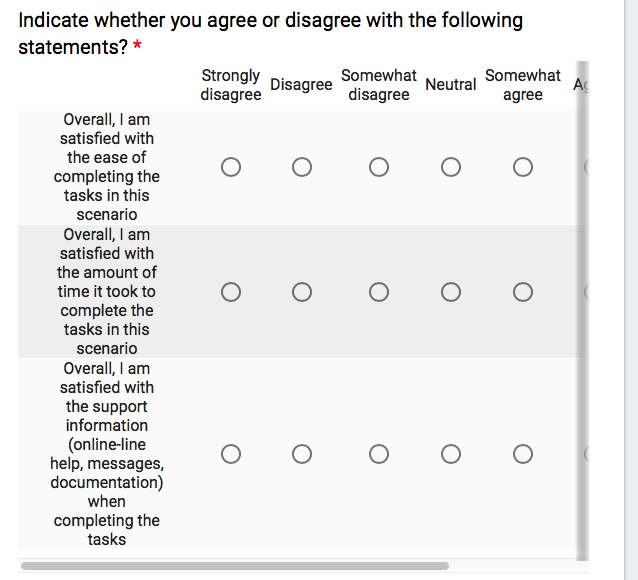
\includegraphics[keepaspectratio=true,scale=0.35]{../resources/images/google-limitation.png}
 }
\captionof{figure}{Google form hiding some options on 7 point scale} \label{fig:google-limit}%      only if needed  
\end{minipage}


\vspace{1cm}
\noindent%
\begin{minipage}{\linewidth}% to keep image and caption on one page
\makebox[\linewidth]{
  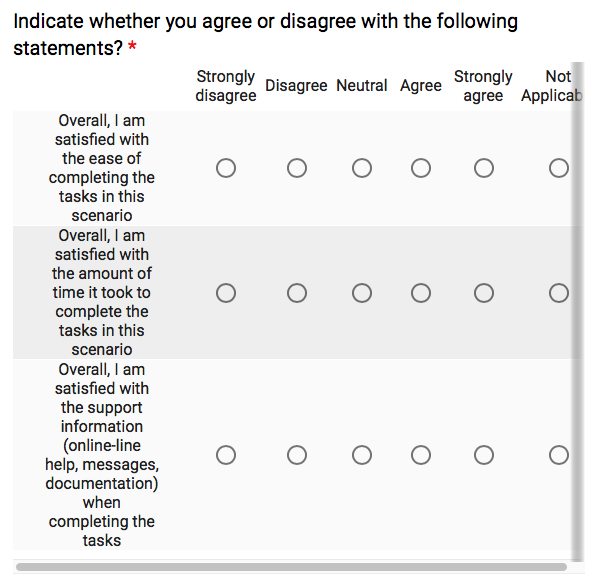
\includegraphics[keepaspectratio=true,scale=0.35]{../resources/images/google-limitation2.png}
 }
\captionof{figure}{Google form render 5 point scale rating better} \label{fig:google-limit2}%      only if needed  
\end{minipage}

\vspace{1cm}


Figure \ref{fig:google-limit} show the limitation of the platform. The response options are not rendered in complete, as in some are hidden in a scrolling element of the page. This leads to respondents have to scroll left and right to see the options and answers. I find this is a detriment to the respondents to do more work in answering the question so I decided to use 5 point scale to make sure everything is rendered better like shown in Figure \ref{fig:google-limit2}.


Another limitation of the study is the way the study compare the experience of doing the scenarios in the questionnaire between using web browser and using command line.  When measuring the usability of HemeWeb, respondents are asked to do the task in the web browser, compared to the task in command line where it is just described in an overview. This decision is made because we cannot make sure the respondents have the necessary tools to run or reproduce a simulation in their computers.  In addition, in order to run the scenario in command line interface, respondents have to install tools on their computer which are timely and prone to errors. I believe this will affect their sentiment in answering the survey questionnaire and decided against it.


\subsection{Performance evaluation}

On running the HemeLB simulation on the three systems compared, we cannot fully isolate the infrastructure from various system load the infrastructure is handling. The performance might be affected by other jobs running in the system, which is apparent in the case of ARCHER supercomputer where many jobs are executing at the same moment. The same case with INDY2. The performance benchmark might be not as accurate as a completely isolated environment, however it paints a pretty good picture of performance you get when using cloud vendors compared to the dedicated infrastructure. 

Also another limitation on the performance evaluation is that we cannot get more than 20 instances of c4.8xlarge instances on AWS. This causes the evaluation for AWS-EC2 cannot be done for the 1,152 cores to compare it directly with INDY2. Another problem is that on ARCHER, it has 24 cores in 1 compute node compared to 36 in INDY2 and AWS-EC2. We wanted to measure the full load of the compute node, therefore we cannot get an exact apple to apple comparison. However, it could help in painting the general trend of the scaling capabilities and measure based on that.
 
